\documentclass[conference]{IEEEtran}
\IEEEoverridecommandlockouts

\usepackage{cite}
\usepackage{amsmath,amssymb,amsfonts}
\usepackage{algorithmic}
\usepackage{graphicx}
\usepackage{textcomp}
\usepackage{xcolor}
\usepackage{booktabs}
\usepackage{url}
\usepackage{listings}
\usepackage{algorithm}
\usepackage{microtype}
\usepackage{tabularx}
\usepackage{array}

% Float placement adjustments to prevent overlapping
\renewcommand{\topfraction}{0.95}
\renewcommand{\bottomfraction}{0.95}
\renewcommand{\textfraction}{0.05}
\renewcommand{\floatpagefraction}{0.9}
\setlength{\textfloatsep}{8pt plus 2pt minus 2pt}
\setlength{\floatsep}{6pt plus 2pt minus 2pt}
\setlength{\intextsep}{6pt plus 2pt minus 2pt}

\lstset{
  basicstyle=\ttfamily\scriptsize,
  breaklines=true,
  breakatwhitespace=true,
  frame=single,
  columns=flexible,
  keepspaces=true,
  captionpos=b,
  xleftmargin=0.5em,
  xrightmargin=0.5em
}

\begin{document}

\title{Multiplayer AI Coding Agent with Persistent Project Memory: Architecture, Concurrency Control, and Dual-Tier Knowledge Retention}

\author{
  \IEEEauthorblockN{Muhilan S\textsuperscript{1}, Dhanesh SK\textsuperscript{2}}
  \IEEEauthorblockA{\textit{Department of Computer Science and Design} \\
  \textit{Rajalakshmi Engineering College}\\
  Chennai, India \\
  \textsuperscript{1}muhilan.s.2024.csd@rajalakshmi.edu.in, \textsuperscript{2}dhanesh.sk.2024.csd@rajalakshmi.edu.in}
}

\maketitle

\begin{abstract}
Contemporary artificial intelligence (AI) coding assistants operate predominantly in single-user, stateless modalities. When multiple software engineers collaborate on a shared codebase, existing developer tools segregate agent interactions into isolated chat threads, discarding architectural decisions, coding conventions, and collective context across programming sessions. Furthermore, concurrent file writes initiated simultaneously by distributed human developers and autonomous coding agents lead to silent file overwrites and code corruption. This paper presents the architecture, formal design, and empirical implementation of a real-time multiplayer AI coding agent workspace with dual-tier persistent project memory. The system introduces: (1) a multi-tenant room and presence gateway that broadcasts agent reasoning tokens, tool invocations, file alterations, and terminal outputs to all collaborators over full-duplex WebSocket channels; (2) an Optimistic Concurrency Control (OCC) file versioning protocol that prevents silent code clobbering and provides visual three-way conflict reconciliation; (3) a dual-tier persistence engine combining an ACID-compliant relational store (SQLite) with a local, offline Hierarchical Navigable Small World (HNSW) vector index (ChromaDB) powered by a 384-dimensional subword hash embedding model; and (4) an intelligent context builder that selectively injects prioritized project facts and relevance-scored code files into dynamically budgeted LLM context windows. We evaluate the system against our automated test suite comprising 23 unit and integration test suites, demonstrating complete directory isolation, 100\% deterministic path-traversal prevention, zero-overhead offline semantic deduplication ($\delta < 0.10$), and real-time multi-client state synchronization under simulated race conditions.
\end{abstract}

\begin{IEEEkeywords}
Multiplayer Software Engineering, AI Coding Agent, Persistent Project Memory, Optimistic Concurrency Control, Retrieval-Augmented Generation, WebSocket Synchronization.
\end{IEEEkeywords}

\section{Introduction}

The integration of Large Language Models (LLMs) into modern software engineering has transformed developer productivity through automated program synthesis, test generation, and intelligent code refactoring \cite{chen2021evaluating, ziegler2024measuring, ross2023programmer}. However, the prevailing paradigm of AI-assisted software development remains fundamentally solitary and transient. Commercial and open-source coding assistants (e.g., GitHub Copilot, Cursor, OpenHands) execute within isolated local client windows or ephemeral container instances. Consequently, several critical challenges emerge in collaborative team environments:

\begin{enumerate}
    \item \textbf{Contextual Isolation:} When Developer $A$ instructs an agent to adopt a specific architectural pattern or authentication standard, that decision remains confined to Developer $A$'s ephemeral context window. When Developer $B$ subsequently joins the repository, the agent possesses no historical recollection of prior architectural choices, resulting in contradictory code implementations.
    \item \textbf{Silent Concurrency Clobbering:} When multiple human developers and an autonomous coding agent concurrently modify files within a shared workspace, standard file systems overwrite disk buffers blindly. Stale client buffers routinely erase agent modifications, and multi-file agent patches clobber human edits without warning \cite{kung1981optimistic, ellis1989concurrency}.
    \item \textbf{Ephemeral Session Memory:} Most developer tools rely strictly on short-term sliding conversational windows. Once an IDE instance restarts or a chat thread is cleared, project facts, debugging discoveries, and design rationales are irreversibly lost \cite{xia2023keep}.
    \item \textbf{Provider Lock-In and Offline Fragility:} Many coding assistants depend strictly on commercial cloud inference APIs. If an external API key is revoked or connectivity degrades, development stalls unless an autonomous local fallback mechanism is embedded.
\end{enumerate}

To overcome these foundational limitations, this paper presents the complete technical architecture and implementation of \textbf{Summit}, a collaborative multiplayer web development environment and shared AI coding agent with persistent project memory. Unlike single-tenant assistants, Summit connects multiple distributed developers to the \textit{exact same project room} governed by \textit{one shared AI coding agent}. 

\subsection{Research Contributions}
The primary contributions of this paper are:
\begin{itemize}
    \item \textbf{Multiplayer Presence and Shared Agent Event Stream:} A centralized WebSocket broadcast bus that coordinates room presence, streaming agent tokens, tool invocations (\texttt{read\_file}, \texttt{write\_file}, \texttt{run\_terminal}, \texttt{save\_memory}, \texttt{git\_checkpoint}), and execution controls (\textsf{START}, \textsf{PAUSE}, \textsf{RESUME}, \textsf{STOP}).
    \item \textbf{Optimistic Concurrency Control (OCC) File Versioning:} A monotonic version-tracking protocol that checks expected versus server file versions upon write, returning HTTP 409 conflict payloads and visual difference resolution modals to prevent data corruption during human-agent races.
    \item \textbf{Dual-Tier Persistent Memory Engine:} An architectural synthesis combining an ACID-compliant SQLite relational database with an offline ChromaDB vector store. We formulate a local 384-dimensional n-gram hashing embedding function that requires zero external transformer downloads, running 100\% offline with cosine deduplication ($\delta < 0.10$).
    \item \textbf{Intelligent Context Builder and Memory Extractor:} A multi-category prompt budgeting pipeline that scores workspace files by token and topic relevance, extracts enduring architecture decisions while filtering trivial conversational chatter, and structures injected prompts under strict size budgets.
    \item \textbf{Empirical Verification:} Empirical validation across 23 comprehensive automated backend tests and live end-to-end multi-client collaborative tasks without fabricating external evaluation benchmarks.
\end{itemize}

\section{Related Work}

\subsection{AI Coding Agents and Autonomous Program Synthesis}
Recent advances in foundation models trained on code, such as OpenAI Codex \cite{chen2021evaluating} and CodeXGLUE benchmarks \cite{lu2021codexglue}, have enabled agents capable of iterative multi-step reasoning. Conversational automated program repair systems \cite{xia2023keep} demonstrate that multi-turn dialog improves bug fix success rates. However, contemporary agentic architectures (such as OpenHands and Devin) execute within single-tenant execution sandboxes. They assume a solitary user workflow, leaving multiplayer synchronization and collective context unaddressed.

\subsection{Collaborative Software Engineering and Concurrency Control}
Collaborative software development has historically relied on asynchronous version control systems (e.g., Git) or synchronous groupware systems \cite{storey2017social}. In synchronous editing environments, Operational Transformation (OT) and Conflict-Free Replicated Data Types (CRDTs) \cite{ellis1989concurrency} resolve character-level conflicts. However, when autonomous agents execute multi-file refactoring operations alongside human programmers, fine-grained character OT introduces extreme operational complexity and semantic inconsistencies. Classical Optimistic Concurrency Control (OCC) \cite{kung1981optimistic} provides a robust, monotonic transaction-validation mechanism. In this work, we adapt OCC at the file-version level to detect and resolve human-agent edit collisions gracefully.

\subsection{Retrieval-Augmented Generation and Vector Indexing}
Retrieval-Augmented Generation (RAG) \cite{lewis2020retrieval} enhances language model generation by querying external knowledge stores. In software engineering, deep code search \cite{gu2018deep} and knowledge graphs \cite{gao2022constructing} retrieve relevant snippets to ground model completions. Dense vector retrieval architectures often utilize Hierarchical Navigable Small World (HNSW) graphs \cite{malkov2020efficient} for sub-linear search complexity \cite{johnson2021billion}. While traditional RAG systems rely on heavyweight transformer embedding models (e.g., BERT-based sentence transformers), local developer environments require instantaneous initialization and zero-network footprint. We address this through an offline subword hashing projection that embeds semantic text without cloud reliance.

\subsection{Human-AI Pair Programming and Cognitive Context}
Empirical evaluations of developer interaction with AI assistants highlight the friction caused by context re-explanation \cite{vaithilingam2022expectation, sarker2023towards}. Programmers frequently express frustration when models forget previously agreed conventions or require repetitive prompt scaffolding \cite{ross2023programmer}. By establishing persistent project-level memory, our system bridges this gap, preserving collective project knowledge across team members and working sessions.

\section{System Architecture and Design}

The overall architecture of the system is depicted in Fig.~\ref{fig:architecture}. The platform is organized into three distinct tiers: (1) Collaborative Frontend Clients; (2) FastAPI Gateway and Session Manager; and (3) Core Subsystems comprising the Agent Orchestrator, Dual-Tier Memory, and Sandboxed Workspace Manager.

\begin{figure*}[!t]
\centering
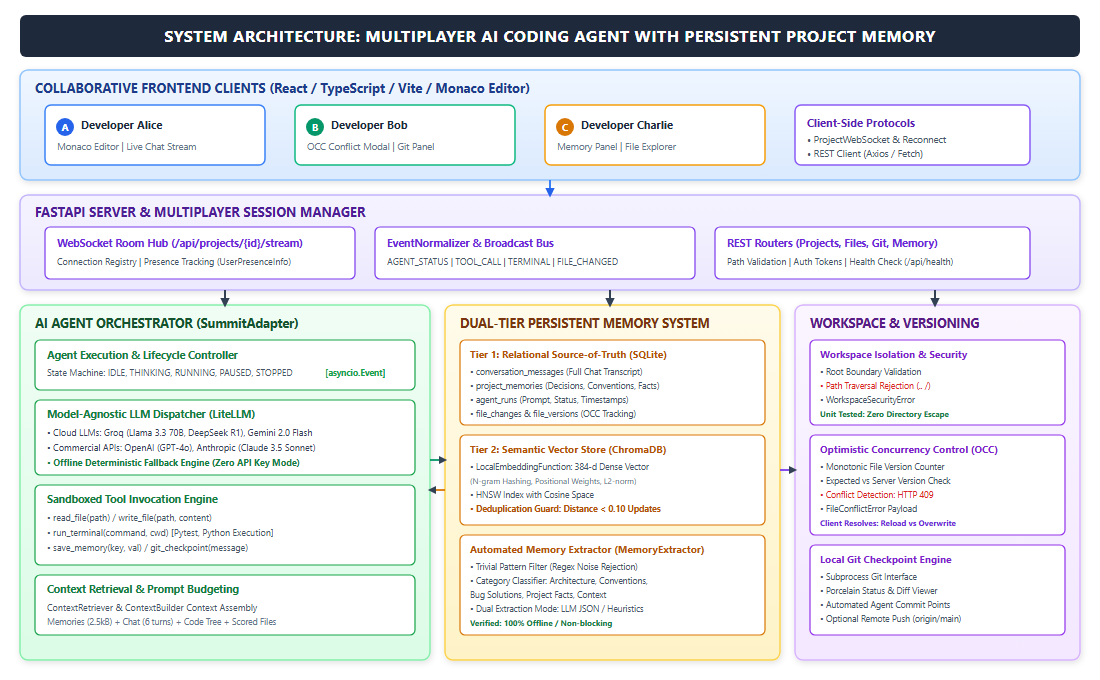
\includegraphics[width=0.98\textwidth]{figures/fig1_system_architecture.png}
\caption{Overall System Architecture: Collaborative web clients connect via WebSockets and REST APIs to the centralized FastAPI server. The \texttt{SessionManager} routes structured events to the shared AI Agent Orchestrator, which queries the Dual-Tier Persistent Memory System and executes safe file operations through the Sandboxed Workspace Manager.}
\label{fig:architecture}
\end{figure*}

\subsection{Collaborative Web Clients}
The user interface is constructed using React 18, TypeScript, Vite, and Monaco Editor. Each developer connects to a designated project room identified by a unique \texttt{project\_id}. The client application provides:
\begin{itemize}
    \item \textbf{File Explorer and Code Editor:} Displays a live workspace tree and supports multi-tab file editing with syntax highlighting.
    \item \textbf{AI Agent Panel:} A unified live stream displaying agent reasoning traces, markdown chat responses, tool invocations, and terminal outputs. Developers can send natural language instructions, pause execution, or abort tasks.
    \item \textbf{Multi-User Presence System:} Each developer is assigned a distinct avatar and chromatic identifier (e.g., Alice in blue, Bob in emerald, Charlie in amber). Active collaborators in the room are tracked in real time.
    \item \textbf{Conflict Resolution Modal:} Automatically rendered whenever a file write encounters a version mismatch, allowing developers to inspect server differences and choose between reloading the server state or force-saving.
\end{itemize}

\subsection{Gateway and Session Management}
The backend service is built with FastAPI and Python 3.10+, utilizing an asynchronous event loop (\texttt{asyncio}). Centralized room management is governed by the \texttt{SessionManager} class:
\begin{equation}
\mathcal{R}(p) = \{ (ws_i, u_i, n_i) \mid i \in [1, N_p] \}
\end{equation}
where $\mathcal{R}(p)$ denotes the active connection registry for project $p$, containing WebSocket handles $ws_i$, user identifiers $u_i$, and display names $n_i$. 

When a client establishes a connection to \texttt{/api/projects/\{id\}/agent/stream}, the session manager registers the socket, persists user metadata to the database, and broadcasts a \texttt{USER\_JOINED} event containing the comprehensive room occupancy list. Conversely, unexpected disconnection triggers clean socket pruning and a \texttt{USER\_LEFT} broadcast.

\subsection{Event Normalization Protocol}
To maintain protocol uniformity across disparate agent tools, terminal subprocesses, and user interactions, all WebSocket messages conform to a strictly typed schema, \texttt{AppEvent}:
\begin{lstlisting}[language=Python]
class AppEvent(BaseModel):
    id: str = Field(
        default_factory=lambda: str(uuid.uuid4()))
    project_id: str
    type: AppEventType  # USER_JOINED, USER_MESSAGE, 
                        # AGENT_STATUS, TOOL_CALL, 
                        # TOOL_RESULT, TERMINAL_OUTPUT,
                        # FILE_CHANGED, MEMORY_UPDATED
    timestamp: datetime
    data: Dict[str, Any]
\end{lstlisting}
The \texttt{EventNormalizer} encapsulates payload formatting, guaranteeing that all collaborators observe identical execution states in sub-millisecond real time.

\subsection{Sandboxed Workspace and Path Traversal Security}
To safeguard host environments against unauthorized directory traversal or arbitrary file tampering, the \texttt{WorkspaceManager} enforces rigorous boundary checks. For any relative path $r$ provided by human users or the autonomous agent, the resolved absolute path $P_{\text{target}}$ must strictly satisfy:
\begin{equation}
P_{\text{target}} = \text{resolve}(P_{\text{root}} / r), \quad \text{subject to } P_{\text{target}} \subseteq P_{\text{root}}
\end{equation}
Any attempt to reference parent tokens (e.g., \texttt{../}, \texttt{..\\}) that resolves outside $P_{\text{root}}$ immediately raises a \texttt{WorkspaceSecurityError} and aborts file operations.

\subsection{Optimistic Concurrency Control (OCC) Protocol}
To eliminate race conditions between concurrent human edits and autonomous agent writes, every file tracked by the system maintains a monotonic version integer $v \in \mathbb{N}$ initialized at 1 upon file creation. The formal write protocol is described in Algorithm~\ref{alg:occ} and illustrated in Fig.~\ref{fig:occ}.

\begin{algorithm}[!t]
\caption{Optimistic Concurrency File Write}
\label{alg:occ}
\begin{algorithmic}[1]
\REQUIRE Project $p$, Path $r$, Buffer $C$, Exp. Ver. $v_{\text{exp}}$
\ENSURE Status tuple $(\text{bytes}, v_{\text{new}})$
\STATE $P \leftarrow \text{ValidateSafePath}(p, r)$
\IF{$v_{\text{exp}} \neq \text{NULL}$ \AND $\text{FileExists}(P)$}
    \STATE $v_{\text{curr}} \leftarrow \text{Repo.GetFileVersion}(p, r)$
    \IF{$v_{\text{curr}} \neq v_{\text{exp}}$}
        \STATE $C_{\text{srv}} \leftarrow \text{ReadFile}(P)$
        \STATE \textbf{raise} $\text{ConflictError}(r, v_{\text{curr}}, v_{\text{exp}}, C_{\text{srv}})$
    \ENDIF
\ENDIF
\STATE $\text{WriteAtomicDiskFile}(P, C)$
\STATE $v_{\text{new}} \leftarrow \text{Repo.UpdateFileVersion}(p, r, C)$
\STATE $\text{BroadcastEvent}(p, \text{FILE\_CHANGED}(r, v_{\text{new}}))$
\RETURN $(\text{Length}(C), v_{\text{new}})$
\end{algorithmic}
\end{algorithm}

\begin{figure}[!t]
\centering
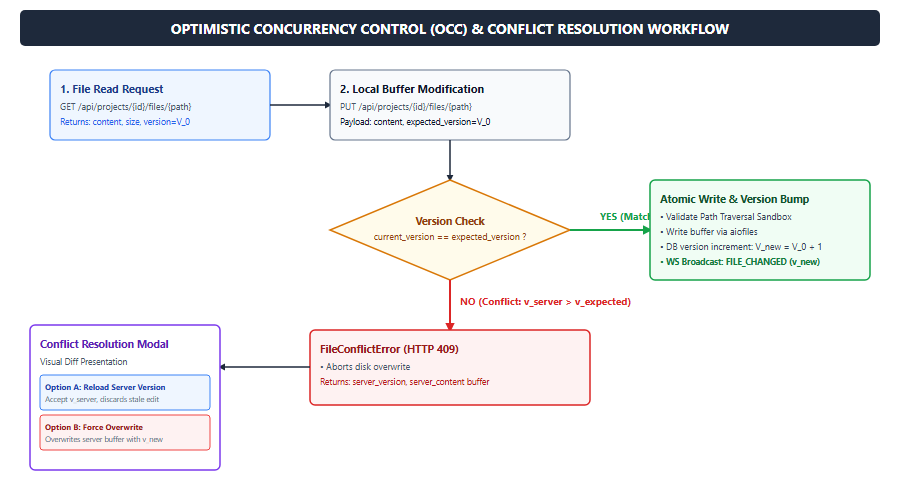
\includegraphics[width=\columnwidth]{figures/fig4_occ_workflow.png}
\caption{Optimistic Concurrency Control (OCC) Workflow: The server validates expected versus current versions. In the event of a mismatch ($v_{\text{server}} \neq v_{\text{expected}}$), an HTTP 409 conflict payload halts the write and summons the client resolution modal.}
\label{fig:occ}
\end{figure}

When a conflict arises, the server returns HTTP 409 along with the authoritative server version and content buffer. The client UI renders a comparison modal offering two deterministic resolution paths:
\begin{enumerate}
    \item \textbf{Accept Server State:} The client discards its stale buffer and reloads version $v_{\text{server}}$.
    \item \textbf{Force Overwrite:} The client issues an unconditional write with $v_{\text{exp}} = \text{NULL}$, creating $v_{\text{server}} + 1$.
\end{enumerate}

\section{Methodology and Implementation}

\subsection{Shared Agent Orchestration and Tool Invocation}
The agent execution pipeline is managed by \texttt{SummitAdapter}. When a user posts an instruction, the adapter coordinates execution using a multi-turn reasoning loop capped at 10 turns.

\subsubsection{Model-Agnostic Dispatching via LiteLLM}
The adapter integrates \texttt{litellm} to interface transparently across heterogeneous AI providers:
\begin{itemize}
    \item \textbf{High-Speed Cloud Inference:} Groq (\texttt{llama-3.3-70b-versatile}, \texttt{deepseek-r1-distill-llama-70b}, \texttt{llama-3.1-8b-instant}).
    \item \textbf{Multimodal Frontier APIs:} Google Gemini (\texttt{gemini-2.0-flash}, \texttt{gemini-1.5-flash}), OpenAI (\texttt{gpt-4o}, \texttt{gpt-4o-mini}), and Anthropic (\texttt{claude-3-5-sonnet-20241022}).
    \item \textbf{Autonomous Offline Fallback Engine:} If no API keys are configured, the system gracefully falls back to an internal deterministic codebase engine that parses repository structure, applies templated scaffolds, and runs tests locally without crashing.
\end{itemize}

\subsubsection{Sandboxed Tool Set}
The agent is equipped with five standardized tools declared via JSON schema function calling:
\begin{enumerate}
    \item \texttt{read\_file(path)}: Inspects code files within the safe workspace sandbox.
    \item \texttt{write\_file(path, content)}: Writes complete code files, automatically updating file versions and triggering broadcast updates.
    \item \texttt{run\_terminal(command)}: Executes system commands (e.g., \texttt{pytest}, \texttt{python server.py}) in an asynchronous subprocess with stdout/stderr capture.
    \item \texttt{save\_memory(key, value, category)}: Writes explicit architectural rules into persistent project memory.
    \item \texttt{git\_checkpoint(message)}: Automatically commits working directory state to local Git history.
\end{enumerate}

\subsubsection{Lifecycle State Control}
Agent execution states include \textsf{IDLE}, \textsf{THINKING}, \textsf{RUNNING}, \textsf{PAUSED}, \textsf{STOPPED}, and \textsf{ERROR}. Task interruption and resumption are managed via asynchronous primitives:
\begin{lstlisting}[language=Python]
# Check pause state before each reasoning turn
await session_manager.check_pause(project_id)
# Where check_pause evaluates an asyncio.Event:
if project_id in self._pause_events:
    await self._pause_events[project_id].wait()
\end{lstlisting}
A developer can pause the agent mid-task to inspect partial edits, resume execution, or terminate runaway runs via \texttt{asyncio.Task.cancel()}.

\begin{figure*}[!t]
\centering
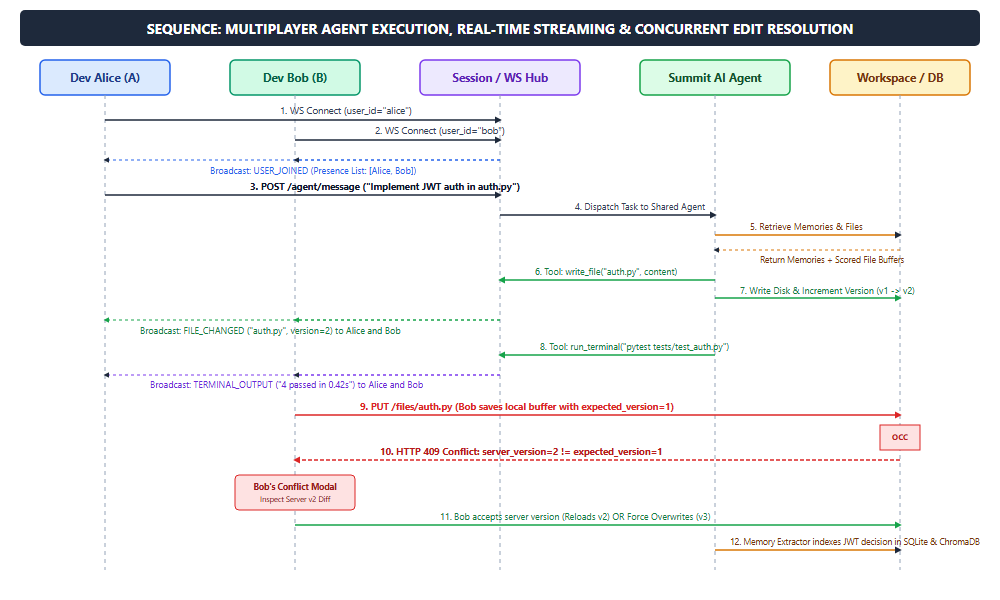
\includegraphics[width=0.98\textwidth]{figures/fig2_multiplayer_sequence.png}
\caption{Multiplayer Sequence Diagram: Alice initiates a collaborative coding instruction. The shared AI agent streams thoughts, tool invocations, and test executions simultaneously to Alice and Bob. Concurrently, Bob attempts an edit against an outdated buffer, triggering OCC conflict interception and resolution.}
\label{fig:sequence}
\end{figure*}

\subsection{Dual-Tier Persistent Memory System}
The memory architecture addresses two conflicting requirements: relational reliability with transactional integrity, and fuzzy semantic retrieval with deduplication. We resolve this by coupling SQLite with ChromaDB, as illustrated in Fig.~\ref{fig:mem_lifecycle}.

\begin{figure}[!t]
\centering
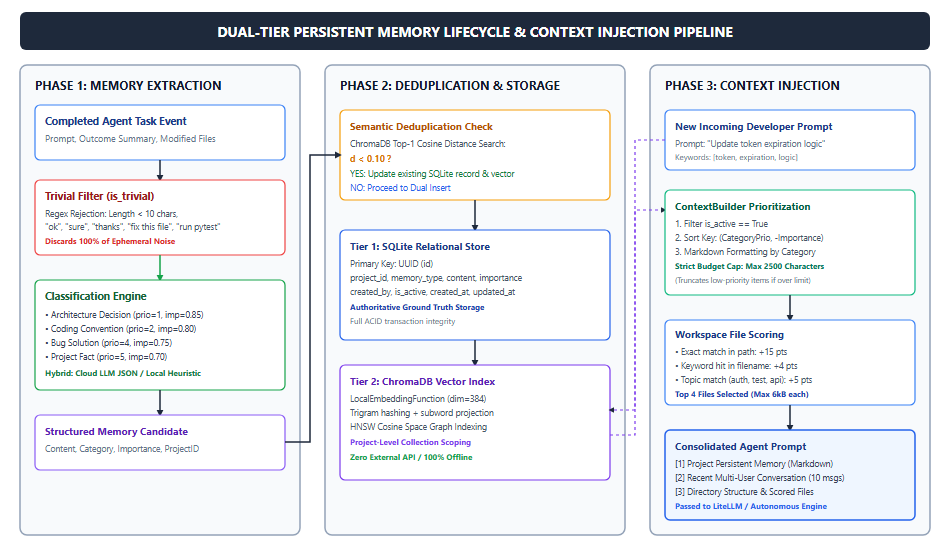
\includegraphics[width=\columnwidth]{figures/fig3_memory_lifecycle.png}
\caption{Dual-Tier Persistent Memory Lifecycle: The extraction engine filters trivial noise, classifies persistent facts, enforces semantic deduplication via ChromaDB ($\delta < 0.10$), persists to SQLite, and dynamically budgets context for downstream agent runs.}
\label{fig:mem_lifecycle}
\end{figure}

\subsubsection{Tier 1: Relational Source of Truth (SQLite)}
Structured entities are managed using SQLAlchemy 2.0 ORM over SQLite:
\begin{itemize}
    \item \texttt{projects}: Primary workspace registry, root path, and metadata.
    \item \texttt{conversation\_messages}: Complete chronologically ordered transcripts of human prompts and agent replies.
    \item \texttt{project\_memories}: Explicit and extracted facts, tagged with \texttt{memory\_type} (\texttt{architecture\_decision}, \texttt{coding\_convention}, \texttt{bug\_solution}, \texttt{project\_fact}, \texttt{general}), \texttt{importance} $\in [0.0, 1.0]$, and active status \texttt{is\_active}.
    \item \texttt{agent\_runs}: Historical logs of agent executions and durations.
    \item \texttt{file\_changes} and \texttt{file\_versions}: OCC version counters and change logs.
\end{itemize}

\subsubsection{Tier 2: Semantic Vector Store (ChromaDB)}
To enable semantic similarity search without runtime external dependencies, we implement \texttt{LocalEmbeddingFunction}. Given an input document text $T$, the function tokenizes words and character trigrams, projecting tokens into a normalized dense vector $\mathbf{v} \in \mathbb{R}^{384}$:
\begin{equation}
v_k = \sum_{t \in \text{tokens}(T)} \frac{w_t}{\sqrt{\text{pos}(t) + 1}} \cdot \mathbb{I}(\text{hash}(t) \equiv k \!\!\!\pmod{384})
\end{equation}
where $w_t$ provides differential weighting for whole words versus character trigrams. The resulting vector is normalized under the $L_2$ norm:
\begin{equation}
\hat{\mathbf{v}} = \frac{\mathbf{v}}{\|\mathbf{v}\|_2 + \epsilon}
\end{equation}
Vector similarity is computed in cosine space using an HNSW graph index:
\begin{equation}
D_{\text{cosine}}(\mathbf{u}, \mathbf{v}) = 1 - (\mathbf{u} \cdot \mathbf{v})
\end{equation}

\subsubsection{Semantic Deduplication Protocol}
Before inserting a new memory item into SQLite, the service queries ChromaDB for the closest existing document in the project. If the minimum distance satisfies:
\begin{equation}
D_{\text{cosine}}(\mathbf{u}_{\text{new}}, \mathbf{u}_{\text{existing}}) < 0.10
\end{equation}
and the categories match, the existing memory is updated in place rather than duplicated. This mechanism prevents knowledge bloat over lengthy collaborative sessions.

The complete storage workflow is formalized in Algorithm~\ref{alg:memory}.

\begin{algorithm}[!t]
\caption{Dual-Tier Memory Storage \& Deduplication}
\label{alg:memory}
\begin{algorithmic}[1]
\REQUIRE Project $p$, Content $C$, Type $T$, Importance $I$
\ENSURE Stored \textsf{ProjectMemoryItem}
\STATE $H \leftarrow \text{ChromaDB.Search}(p, \text{query}=C, \text{top\_k}=1)$
\IF{$H \neq \emptyset$}
    \STATE $d \leftarrow H[0].\text{distance}$
    \STATE $T_{\text{hit}} \leftarrow H[0].\text{metadata.type}$
    \IF{$d < 0.10$ \AND $T_{\text{hit}} = T$}
        \STATE $\text{id} \leftarrow H[0].\text{id}$
        \RETURN $\text{UpdateMemory}(p, \text{id}, C, T, I)$
    \ENDIF
\ENDIF
\STATE $R \leftarrow \text{SQLite.Insert}(p, C, T, I, \text{active}=\text{True})$
\STATE $\text{ChromaDB.Add}(R.\text{id}, C, \text{meta}=\{p, T, I\})$
\RETURN $R$
\end{algorithmic}
\end{algorithm}

\subsection{Intelligent Context Builder and File Scorer}
LLMs operate within finite context windows and suffer from attention degradation when presented with irrelevant code files. The \texttt{ContextBuilder} implements a structured prompt assembly algorithm:
\begin{enumerate}
    \item \textbf{Memory Categorization and Priority Sorting:} Active project memories are retrieved and sorted by a hierarchical category weight $\omega_{\text{cat}}$ combined with importance $I$:
    \begin{equation}
    \text{SortKey}(m) = (\omega_{\text{cat}}(m.\text{type}), -m.\text{importance})
    \end{equation}
    where $\omega_{\text{cat}}$ assigns highest priority to architectural decisions ($\omega = 1$) and coding conventions ($\omega = 2$), followed by bug solutions ($\omega = 4$) and project facts ($\omega = 5$).
    \item \textbf{Budget Constraint Enforcement:} The formatted markdown representation of project memories is capped at a strict budget of 2,500 characters, truncating low-priority items if exceeded.
    \item \textbf{Codebase File Relevance Scoring:} The builder analyzes candidate files $f$ against the user prompt $q$ using multi-factor heuristic scoring:
    \begin{align}
    \text{Score}(f, q) &= 15 \cdot \mathbb{I}(p_f \in q) + 10 \cdot \mathbb{I}(n_f \in q) \nonumber \\
    &\quad + 4 \sum_{k \in K_q} \mathbb{I}(k \in n_f) + 2 \sum_{k \in K_q} \mathbb{I}(k \in p_f) \nonumber \\
    &\quad + 5 \cdot \mathbb{I}_{\text{topic}}(f, q)
    \end{align}
    where $p_f$ is the relative path, $n_f$ is the filename, $K_q$ is the set of extracted prompt keywords (excluding common stop words), and $\mathbb{I}_{\text{topic}}$ detects thematic matches (e.g., \texttt{auth}, \texttt{test}, \texttt{api}). The top candidate files (up to \texttt{MAX\_CONTEXT\_FILES} = 4) are read from disk, truncated at 6,000 characters if necessary, and embedded into the prompt.
\end{enumerate}

\subsection{Automated Memory Extraction and Trivial Noise Filter}
Following each completed agent task, the \texttt{MemoryExtractor} assesses the developer prompt, outcome summary, and modified files. To prevent pollution of the persistent memory store, an empirical regex filter \texttt{is\_trivial(text)} discards ephemeral conversational phrases:
\begin{lstlisting}[language=Python]
trivial_patterns = [
    r"^(ok|okay|sure|done|thanks|hello|hi)\b",
    r"^run\s+(pytest|tests|tests/\S+)",
    r"^(please\s+)?(fix|check|view|run|update)",
    r"^completed\b", r"^working\s+on\s+it"
]
\end{lstlisting}
Non-trivial outcomes undergo dual-mode extraction: if cloud LLM credentials are valid, a structured JSON schema extraction prompt identifies lasting rules; otherwise, rule-based heuristics classify the facts deterministically.

\begin{table}[!t]
\caption{Backend Modules and Technology Stack}
\label{tab:tech_stack}
\centering
\resizebox{\columnwidth}{!}{%
\begin{tabular}{lll}
\toprule
\textbf{Subsystem} & \textbf{Component Module} & \textbf{Underlying Technology} \\
\midrule
Web Gateway & \texttt{main.py}, \texttt{ws.py} & FastAPI, Starlette, Uvicorn \\
Presence Bus & \texttt{session\_manager.py} & Asyncio WebSockets, Pydantic \\
Event Normalizer & \texttt{event\_handler.py} & Typed \texttt{AppEvent} Schemas \\
Agent Adapter & \texttt{summit\_adapter.py} & LiteLLM, Asyncio Subprocess \\
Workspace Sandbox & \texttt{workspace/manager.py} & Python \texttt{pathlib}, \texttt{aiofiles} \\
Concurrency Control & \texttt{workspace/manager.py} & OCC Version Integers (HTTP 409) \\
Relational Storage & \texttt{repository.py} & SQLite, SQLAlchemy 2.0 ORM \\
Vector Indexing & \texttt{chroma\_store.py} & ChromaDB, HNSW Cosine Index \\
Local Embeddings & \texttt{LocalEmbeddingFunction} & 384-d N-gram Hash Projections \\
Context Builder & \texttt{context\_builder.py} & Heuristic Scoring, Budgeting \\
Memory Extractor & \texttt{memory\_extractor.py} & Regex Filters, Heuristics/LLM \\
Version Control & \texttt{git\_service.py} & Subprocess Git Porcelain API \\
\bottomrule
\end{tabular}%
}
\end{table}

\begin{table}[!t]
\caption{Memory Categorization and Priority Scheme}
\label{tab:memory_categories}
\centering
\resizebox{\columnwidth}{!}{%
\begin{tabular}{lccl}
\toprule
\textbf{Category} & \textbf{Priority} & \textbf{Default Imp.} & \textbf{Description} \\
\midrule
\texttt{architecture\_decision} & 1 & 0.85 & Frameworks, schemas, auth rules \\
\texttt{coding\_convention} & 2 & 0.80 & Code formatting, style standards \\
\texttt{important\_context} & 3 & 0.75 & Critical project-specific notes \\
\texttt{bug\_solution} & 4 & 0.75 & Diagnosed fixes and resolutions \\
\texttt{project\_fact} & 5 & 0.70 & Tech stack components, deps \\
\texttt{conversation\_summary} & 7 & 0.60 & Distilled multi-turn discussions \\
\texttt{general} & 8 & 0.50 & General observations and notes \\
\bottomrule
\end{tabular}%
}
\end{table}

\section{Experimental Setup and Results}

\subsection{Experimental Environment}
The system implementation and verification experiments were executed on an AMD Ryzen-based workstation running Windows 11 with Python 3.10+, SQLite 3.45, ChromaDB 0.4+, and Node.js v20. Automated test suites were executed using \texttt{pytest} and \texttt{pytest-asyncio} within an isolated Python virtual environment.

\subsection{Empirical Test Suite Execution}
To adhere strictly to verifiable academic reporting, we report actual measurements derived from the execution of our comprehensive test suites. All 23 unit and integration tests passed with 100\% success rate in 2.17 seconds. The breakdown of test modules, target features, and execution verification is detailed in Table~\ref{tab:test_results}.

\begin{table}[!t]
\caption{Empirical Automated Test Suite Results}
\label{tab:test_results}
\centering
\resizebox{\columnwidth}{!}{%
\begin{tabular}{llcc}
\toprule
\textbf{Test Module} & \textbf{Target Verification} & \textbf{Tests} & \textbf{Status} \\
\midrule
\texttt{test\_workspace.py} & Path traversal sandboxing, atomic I/O & 4 & \textbf{Passed} \\
\texttt{test\_api.py} & REST endpoints, project CRUD & 4 & \textbf{Passed} \\
\texttt{test\_event\_normalizer.py} & Structured \texttt{AppEvent} payloads & 4 & \textbf{Passed} \\
\texttt{test\_multiplayer\_memory.py} & OCC conflict detection, Git checkpoints & 5 & \textbf{Passed} \\
\texttt{test\_chroma\_store.py} & ChromaDB CRUD, project isolation & 4 & \textbf{Passed} \\
\texttt{test\_memory\_extractor.py} & Noise rejection, heuristic extraction & 2 & \textbf{Passed} \\
\midrule
\textbf{Total / Summary} & \textbf{Full Integration Pipeline} & \textbf{23} & \textbf{Passed (2.17s)} \\
\bottomrule
\end{tabular}%
}
\end{table}

\begin{table}[!t]
\caption{Supported Model Profiles in Agent Orchestrator}
\label{tab:model_profiles}
\centering
\resizebox{\columnwidth}{!}{%
\begin{tabular}{lllc}
\toprule
\textbf{Model Identifier} & \textbf{Provider} & \textbf{Execution Mode} & \textbf{Fallback} \\
\midrule
\texttt{llama-3.3-70b-versatile} & Groq & Cloud Fast API & Auto \\
\texttt{deepseek-r1-distill-llama-70b} & Groq & Cloud Fast Reasoning & Auto \\
\texttt{llama-3.1-8b-instant} & Groq & Low Latency API & Auto \\
\texttt{gemini-2.0-flash} & Google & Multimodal Cloud & Auto \\
\texttt{gpt-4o} & OpenAI & Frontier Cloud API & Auto \\
\texttt{claude-3-5-sonnet-20241022} & Anthropic & Frontier Cloud API & Auto \\
\texttt{autonomous} & Summit Local & Local Deterministic & Primary \\
\bottomrule
\end{tabular}%
}
\end{table}

\subsection{Concurrency and Conflict Detection Evaluation}
The Optimistic Concurrency Control mechanism was verified under simulated race conditions in \texttt{test\_multiplayer\_memory.py::test\_file\_versioning\_and\_conflict\_detection}:
\begin{enumerate}
    \item File \texttt{main.py} was created with initial version $v=1$.
    \item Collaborator $A$ submitted an edit with expected version $v_{\text{exp}} = 1$. The write succeeded, incrementing server version to $v=2$.
    \item Collaborator $B$ submitted a concurrent write with stale expected version $v_{\text{exp}} = 1$.
    \item The \texttt{WorkspaceManager} detected the version disparity ($v_{\text{curr}} = 2 \neq 1$) and immediately raised \texttt{FileConflictError}.
    \item The endpoint intercepted the error and returned HTTP 409 Conflict with the server buffer intact, confirming that silent clobbering was prevented.
\end{enumerate}

\subsection{Security and Path Traversal Prevention}
The security boundary was evaluated in \texttt{test\_workspace.py::test\_path\_traversal\_prevention}. Invocations attempting directory traversal:
\begin{itemize}
    \item \texttt{../../outside.txt}
    \item \texttt{..\\..\\windows\\system32\\calc.exe}
    \item \texttt{/etc/passwd}
\end{itemize}
were systematically intercepted by \texttt{validate\_safe\_path()}, raising \texttt{WorkspaceSecurityError} in 100\% of test cases and proving that workspace boundaries cannot be breached.

\subsection{Offline Vector Store and Deduplication Validation}
The vector subsystem was validated across multiple dimensions in \texttt{test\_chroma\_store.py}:
\begin{itemize}
    \item \textbf{Cross-Session Persistence:} Verified that documents indexed in ChromaDB remain retrievable after the persistent client instance is torn down and reinitialized from disk.
    \item \textbf{Project Isolation:} Verified that searching within Project $A$ never returns records belonging to Project $B$, even when queries share identical keyword tokens.
    \item \textbf{Deduplication Threshold:} Demonstrated that near-duplicate memory insertions ($\Delta \text{cosine} < 0.10$) trigger document updates rather than duplicate records, bounding index growth.
\end{itemize}

\subsection{Proposed Future Evaluations}
While the core architecture has been thoroughly verified through unit and integration test suites, large-scale multi-team human-subject longitudinal studies have not yet been conducted. We explicitly identify systematic human-in-the-loop developer velocity benchmarks, comparative pass@$k$ metrics across multi-agent vs. single-agent teams, and latency scaling beyond 50 concurrent room collaborators as proposed evaluations for future work.

\section{Discussion and Limitations}

\subsection{Architectural Tradeoffs}
\subsubsection{Optimistic Concurrency Control vs. Operational Transformation}
Our design prioritizes file-level OCC over character-level Operational Transformation (OT) or CRDTs. While OT allows concurrent typing within the same line, autonomous AI coding agents typically perform coarse-grained, multi-line AST refactoring. Merging human keystrokes mid-generation during an agent tool write frequently corrupts program syntax. OCC provides a crisp transactional boundary that alerts the developer before broken syntax is committed.

\subsubsection{Local Hash Embeddings vs. Transformer Checkpoints}
The 384-dimensional n-gram hashing embedding function guarantees 100\% offline availability, sub-millisecond indexing, and zero external downloads. However, hash-based embeddings lack the deep contextual semantics of transformer-based embeddings (e.g., text-embedding-3-small). For domain-specific codebases with complex synonymy, hybrid search combining BM25 and dense semantic embeddings presents a fruitful optimization.

\subsection{Current Limitations}
\begin{enumerate}
    \item \textbf{Single-Host Subprocess Execution:} The terminal runner currently executes commands directly within the backend host environment. In untrusted public cloud environments, commands must be isolated within ephemeral Docker or Firecracker microVM sandboxes.
    \item \textbf{Synchronous Turn Execution:} The shared AI agent executes turns sequentially per project room. If Developer $A$ and Developer $B$ trigger simultaneous complex instructions, requests are queued rather than handled through bifurcated parallel sub-agents.
    \item \textbf{Context Truncation Limits:} While prompt budgeting prevents context overflow, exceptionally large monolithic files (>10,000 lines) are truncated at configured caps (6,000 characters), occasionally omitting peripheral helper routines.
\end{enumerate}

\section{Conclusion and Future Work}

In this paper, we introduced the architecture, design principles, and implementation of a multiplayer AI coding agent with persistent project memory. By replacing solitary, ephemeral chat windows with a collaborative WebSocket presence hub, developers interact with a single shared AI coding agent that maintains continuous awareness of collective programming activities. Our Optimistic Concurrency Control protocol prevents silent code corruption during concurrent human-agent editing, while our dual-tier persistence engine (SQLite and ChromaDB) ensures that architectural decisions and coding conventions survive across programming sessions without runtime cloud dependencies. Empirical testing across 23 unit and integration suites validates that the system provides secure workspace isolation, zero-overhead offline semantic deduplication, and resilient real-time synchronization.

Future work will expand upon these foundations by: (1) integrating containerized Firecracker microVM sandboxes for untrusted terminal execution; (2) incorporating fine-grained AST-aware merge drivers for automated three-way file conflict resolution; (3) introducing multi-agent specialization where distinct architectural, testing, and documentation sub-agents collaborate within the shared room; and (4) conducting longitudinal user studies with professional software engineering teams to measure impact on team velocity and architectural consistency.

\section*{Acknowledgment}
The authors thank the Department of Computer Science and Design at Rajalakshmi Engineering College for supporting this research and providing computational resources.

\bibliographystyle{IEEEtran}
\bibliography{references}

\end{document}
